Der Standalone Server ohne Datenbank soll für die manuellen Tests der Software der Ladesäule benutzt werden. 
Die Ladesäulesoftware und der Server sollen auf einem Rechner laufen und das Ziel des Einsatzes des Servers ist 
die Funktionalitäten der Ladesäulesoftware zu überprüfen. Der Server soll schnell zu installieren sein und keine externen 
Abhängigkeiten haben.

Die Anforderungen an Standalone Server ohne Datenbank sind:
\begin{itemize}
    \item Datenbank darf nicht benutzt werden.
    \item Gleiche Funktionalität wie bei dem Standalone Server mit Datenbank (siehe Kapitel \ref{kap:taskDescription:standaloneWithDB})
\end{itemize}

Die nachfolgende Abbildung \ref{fig:summaryDiagrammStandaloneWithoutDB} ist ein Übersichtdiagramm der Standalone-Anwendung ohne Datenbank.
\begin{figure}[H]
    \centering
    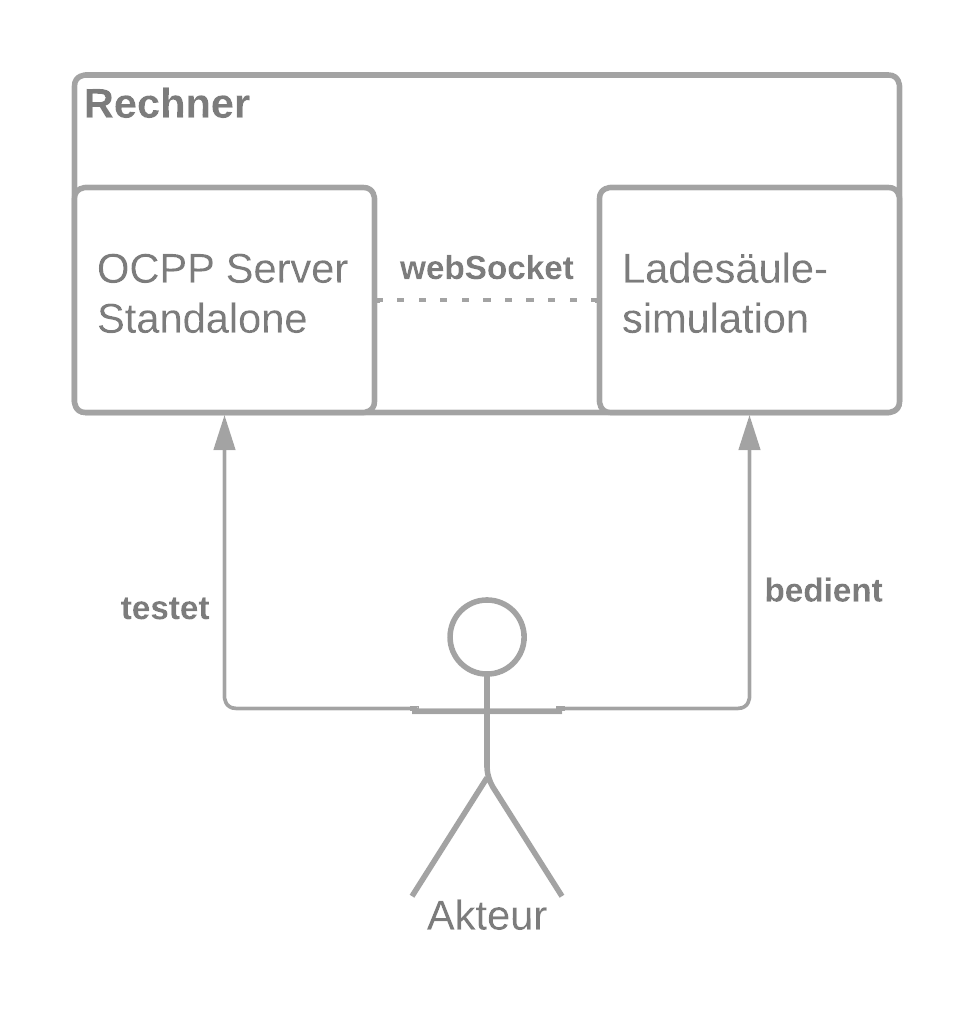
\includegraphics[width=0.5\textwidth]{./images/OCPP Server Standalone ohne DB.png}
    \caption[Übersichtdiagramm der Standalone-Anwendung ohne Datenbank]{Übersichtdiagramm der Standalone-Anwendung ohne Datenbank}
    \label{fig:summaryDiagrammStandaloneWithoutDB}
\end{figure}